\chapter{Introduction}



The fraction of irradiation reflected by Earth's surface is called the albedo. It is linked with the composition and properties of the surface and therefore varies throughout the year. The average albedo for the whole planet is between $0.1$ and $0.3$. Using "ERA5-Land monthly averaged data from 1950 to present" from the Copernicus datastore \citep{hersbach2020era5}, it is possible to retrieve the variable "forecast albedo", which is defined as \textit{the fraction of solar (shortwave) radiation reflected by Earth's surface, across the solar spectrum, for both direct and diffuse radiation}. The figure \ref{fig:avg_albedo} represent monthly averaged albedo value from 1993 to 2022. 

\begin{figure}[ht]
	\centering
	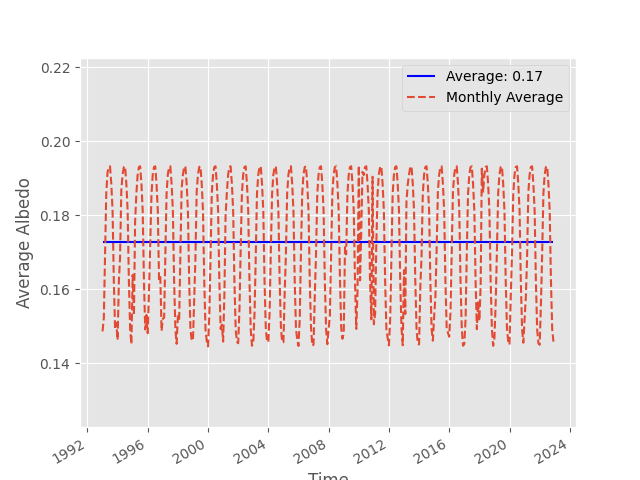
\includegraphics[width=8cm]{albedo_avg_clim}
	\caption{Average value over Ireland from 1993 to 2022}
	\label{fig:avg_albedo}
\end{figure}



